\documentclass{article}

\usepackage{graphicx}
\usepackage{hyperref}
\usepackage{bm}

\usepackage{listings}
\usepackage{color}

\definecolor{dkgreen}{rgb}{0,0.6,0}
\definecolor{gray}{rgb}{0.5,0.5,0.5}
\definecolor{mauve}{rgb}{0.86,0.27,0.22}

\lstset{frame=tb,
  language=python,
  aboveskip=3mm,
  belowskip=3mm,
  showstringspaces=false,
  columns=flexible,
  basicstyle={\small\ttfamily},
  numbers=none,
  numberstyle=\tiny\color{gray},
  keywordstyle=\color{blue},
  commentstyle=\color{dkgreen},
  stringstyle=\color{mauve},
  breaklines=true,
  breakatwhitespace=true,
  tabsize=3
}

%----------------------------------------------------------------------------------------
%	ASSIGNMENT INFORMATION
%----------------------------------------------------------------------------------------

\title{CS5200: Homework \#1} % Title of the assignment

\author{Matthew Whitesides\\ \texttt{mbwxd4@mst.edu}} % Author name and email address

\date{\today} % University, school and/or department name(s) and a date

%----------------------------------------------------------------------------------------

\begin{document}

\maketitle % Print the title
 
\begin{enumerate}
  \item Signed statement on last page. 
  
  \item Question 2.
  \begin{enumerate}
    \item The age of the Earth is estimated at least 4.3 and commonly estimated at \textbf{4.54 billion years} old.

    \item The age of the Solar System is estimated between \textbf{4.53 and 4.58 billion years} old.

    \item The age of the Milky Way Galaxy is estimated at \textbf{11 to 13 billion years} old.

    \item The age of the universe is estimated at \textbf{10 to 15 billion years} old.
    \begin{itemize}
      \bibitem{usgs} 
      (Questions A - D): Dalrymple, G. Brent.
      \textit{The Age of the Earth}.
      \textit{\href{https://pubs.usgs.gov/gip/geotime/age.html}{https://pubs.usgs.gov/gip/geotime/age.html}}
      Stanford University Press, 492p, 1991.
    \end{itemize}

    \item The fate of the earth will probably be ended by our sun expanding into the earth in about 7 billion years putting the earth's lifespan at around \textbf{11 billion years} old.
    \begin{itemize}
      \bibitem{Ward} 
      Ward, Peter.
      \textit{The life and death of planet Earth}.      
      Holt, First edition, page 158, January 1, 2004.
    \end{itemize}

    \item There are many ways earth could become uninhabitable by humans however ignoring man-made disasters, and unplanned events such as an asteroid, the earth will naturally go through temperature cycles that would destroy civilization. A man killing ice age is hard to predict but could begin anywhere from \textbf{one to tens of thousands of years} from now, or millions, the last one was only 11 thousand years ago. Recent human activities have increased the climate decay and instability, and to preserve the climate as long as possible we would need to reduce our carbon emissions, and possibly on the survival of the species perspective would eventually need to figure out ways to massively heat or cool the earth survive natural global temperature cycles.
    \begin{itemize}
      \bibitem{Revkin} 
      Revkin, Andrew C.
      \textit{When Will the Next Ice Age Begin?}.
      \textit{\href{https://www.nytimes.com/2003/11/11/science/when-will-the-next-ice-age-begin.html}{https://www.nytimes.com/2003/11/11/science/when-will-the-next-ice-age-begin.html}}
      New York Times, Nov. 10, 2003, Section F, Page 6.
    \end{itemize}
    \begin{itemize}
      \bibitem{William} 
      Reville, William.
      \textit{How long will the human species survive on Earth?}.
      \textit{\href{https://www.irishtimes.com/news/science/how-long-will-the-human-species-survive-on-earth-1.2885564}{https://www.irishtimes.com/news/science/how-long-will-the-human-species-survive-on-earth-1.2885564}}
      Thu, Dec 8, 2016.
    \end{itemize}

    \item The estimated lifespan of the solar system will be about \textbf{11 billion years}. In around five billion years from now, the sun will enter a red giant phase and slowly expand outward for another billion years before exhausting all its energy.
    \begin{itemize}
      \bibitem{Redd} 
      Redd, Nola Taylor.
      \textit{Red Giant Stars: Facts, Definition and the Future of the Sun}.
      Schröder, Connon Smith, R. (2008).
    \end{itemize}

    \item There are many theories about how the universe will end but a commonly used one is related to heat death. In anywhere from \textbf{1 to 100 trillion years}, there will not be enough matter/energy for stars to form and the universe will contain mainly black holes which themselves will disappear eventually.
    \begin{itemize}
      \bibitem{Yun} 
      Wang, Yun.
      \textit{RCurrent observational constraints on cosmic doomsday}.
      Journal of Cosmology and Astro-Particle Physics. 2004 (12)
    \end{itemize}

    \item If there are 31536000 seconds in a year then (($2^{64}$ - 1) / 31536000) is equal to about \textbf{585 billion years} wich if we go with the lower estimate of the universe lifespan is around \textbf{59\%}.
  \end{enumerate}

  \item Question 3. 
  \begin{enumerate}
    \item Assuming the letters can be used more than once we'd have $26^{9}$ combinations or \textbf{5.43 trillion}.
    \item Using the same logic we'd have \bm{$K^{9}$} \textbf{combinations}.
    \item So if $K^{9} = 9000000000$ then $K = \sqrt[9]{9000000000}$, so $K = 12.765$ or you'd need a \textbf{13 character} alphabet to work.
    \item \bm{$K\times (K - 1)^{n - 1}$}. Pretty much it's the same except the first character is K possible letters and every other character is K - 1 possibilities.
    \item Assuming we're going with small but not trying to min/max the use of paper too much, if we use 10px font, standard 8.5 x 11 letter size (not double sided), at 300px/inch printing, with a small margin of 2px between lines we'll get $(11\times 300) / 12 = 275$ words per page. So \textbf{9 billion / 275 = 32.7 million pages}.
    \item Looking at Amazon I see I can get Amazon Basics paper 5,000 sheets for \$44.99. So $(32700000 / 5000) * 44.99 = 294234.6$ so it'd be a cool \textbf{\$294,234.60} assuming Amazon will sell us 6,540 boxes of paper. Now the best selling file cabinet I see on Amazon is a 3 drawer, 18 inch deep cabinet. Amazon lists the same paper in a 500 sheet reem as being 2 inches thick so we could get $(250\times 18)\times 3 = 13500$ per cabinet. So we'd need $32700000 / 13500 = 2422.22$ or \textbf{2,423} cabinets.
    \item They planned on about \textbf{15 thousand} years to finish the project. However they didn't say how many people would be working on it for that estimate so we can only assume it'd take one person that long. If they hope to finish the project in one persons lifespan given they start at 18 years old and retire at 60 years old (42 years per person) and assuming they accounted for the person working probably wouldn't work 24/7 in that original estimate, they'd need \bm{$15000 / 42 = 357.14$} people (maybe a part time person for the 0.14).
    \item The computer people estimated \textbf{one thousand} days (or 86400000 seconds) to finish, and saying there's 9 billion combinations (which isn't exact but they didn't give all details about their alphabet in the story) it'd have to do \bm{$86400000 / 9000000000 = 0.0096$} \textbf{words/sec} which seems fast but maybe they print inline and on a large sheet with laser printers. 
    \item Good story, I like the Twilight Zone kinda ending. Although seems odd they'd be that afraid of Monks at the end. Does make you think about how little you use large numbers in everday life and how futile it'd be to try to do an entire large task without breaking it down into small peices. Really anything over a 100 or so becomes nonsense in most peoples mind I feel.
  \end{enumerate}

  \item 
  \begin{lstlisting}
    # Problem 1.
    def altDif(n):
        if not n:
            return 0
        return n[0] - altDif(n[1:])

    altDif([3, 5, 4])
    # Out: 2
  \end{lstlisting}

  \item 
  \begin{lstlisting}
    # Problem 6
    def f35qV2(n):
        if n < 8:
            return 'Error'
        elif 0 == n % 5:
            return (0, n / 5)
        elif 1 == n % 5:
            return (2, (n - 6) / 5)
        elif 2 == n % 5:
            return (4, (n - 12) / 5)
        elif 3 == n % 5:
            return (1, (n - 3) / 5)    
        else:
            return (3, (n - 9) / 5)

    # Output:
    for i in range(8, 15):
        print(str(i) + ': ' + str(f35qV2(i)))

        8: (1, 1.0)
        9: (3, 0.0)
        10: (0, 2.0)
        11: (2, 1.0)
        12: (4, 0.0)
        13: (1, 2.0)
        14: (3, 1.0)   
  \end{lstlisting}

  \item 
  \begin{lstlisting}
    # Problem 7
    def f(n):
        if n > 100:
            return n - 10
        else:
            return f(f(n + 11))

    # Output
    for i in [1, -6, 200, 27]:
        print(str(i) + ': ' + str(f(i)))

        1: 91
        -6: 91
        200: 190
        27: 91            
  \end{lstlisting}

  So if you take away the second level of recurison and just try f(n + 11) it's easier to tell what's going on. The overall function won't return until we get a number higher than 100. So we'll keep calling (n + 11) until n is greater than 100. So for this simplier function n = 0 will just keep adding 11 until we hit 110 after ten iterations (then the final answer will be 110 - 10 or 100) and then starting at 1 will also take 10 iterations to get to 111 and leave us with 101. However starting at 2 we'll get there in 9 steps giving us 91 and adding one until n = (11 + 2) or 13 where the process repeats until n is natually greater than 100. Now when we add a second layer of recursion really we're just calling the deepest layer until it returns a number greater than 100 which happens first at (n = 2, 13, 24, 35, etc) which is 101 - 10 or 91. So every n <= 100 is just 91.

  \begin{lstlisting}
    def fV2(n):
      return 91 if n < 101 else n - 10        
  \end{lstlisting}

  So given my explination above how just f(n - 11) works f(f(n + 11)) will always return 91 when the value is less than 101 and we know the rest of the conditions are just (n - 10) and recall by definition n is a whole integer.

  But really the simple rule is f(n) equals 91 when n \textless 101 otherwise f equals (n - 10).

  \item 
    Working it out looks like there are a total of \textbf{65} calls to A() in A(2,2).
    \linebreak
    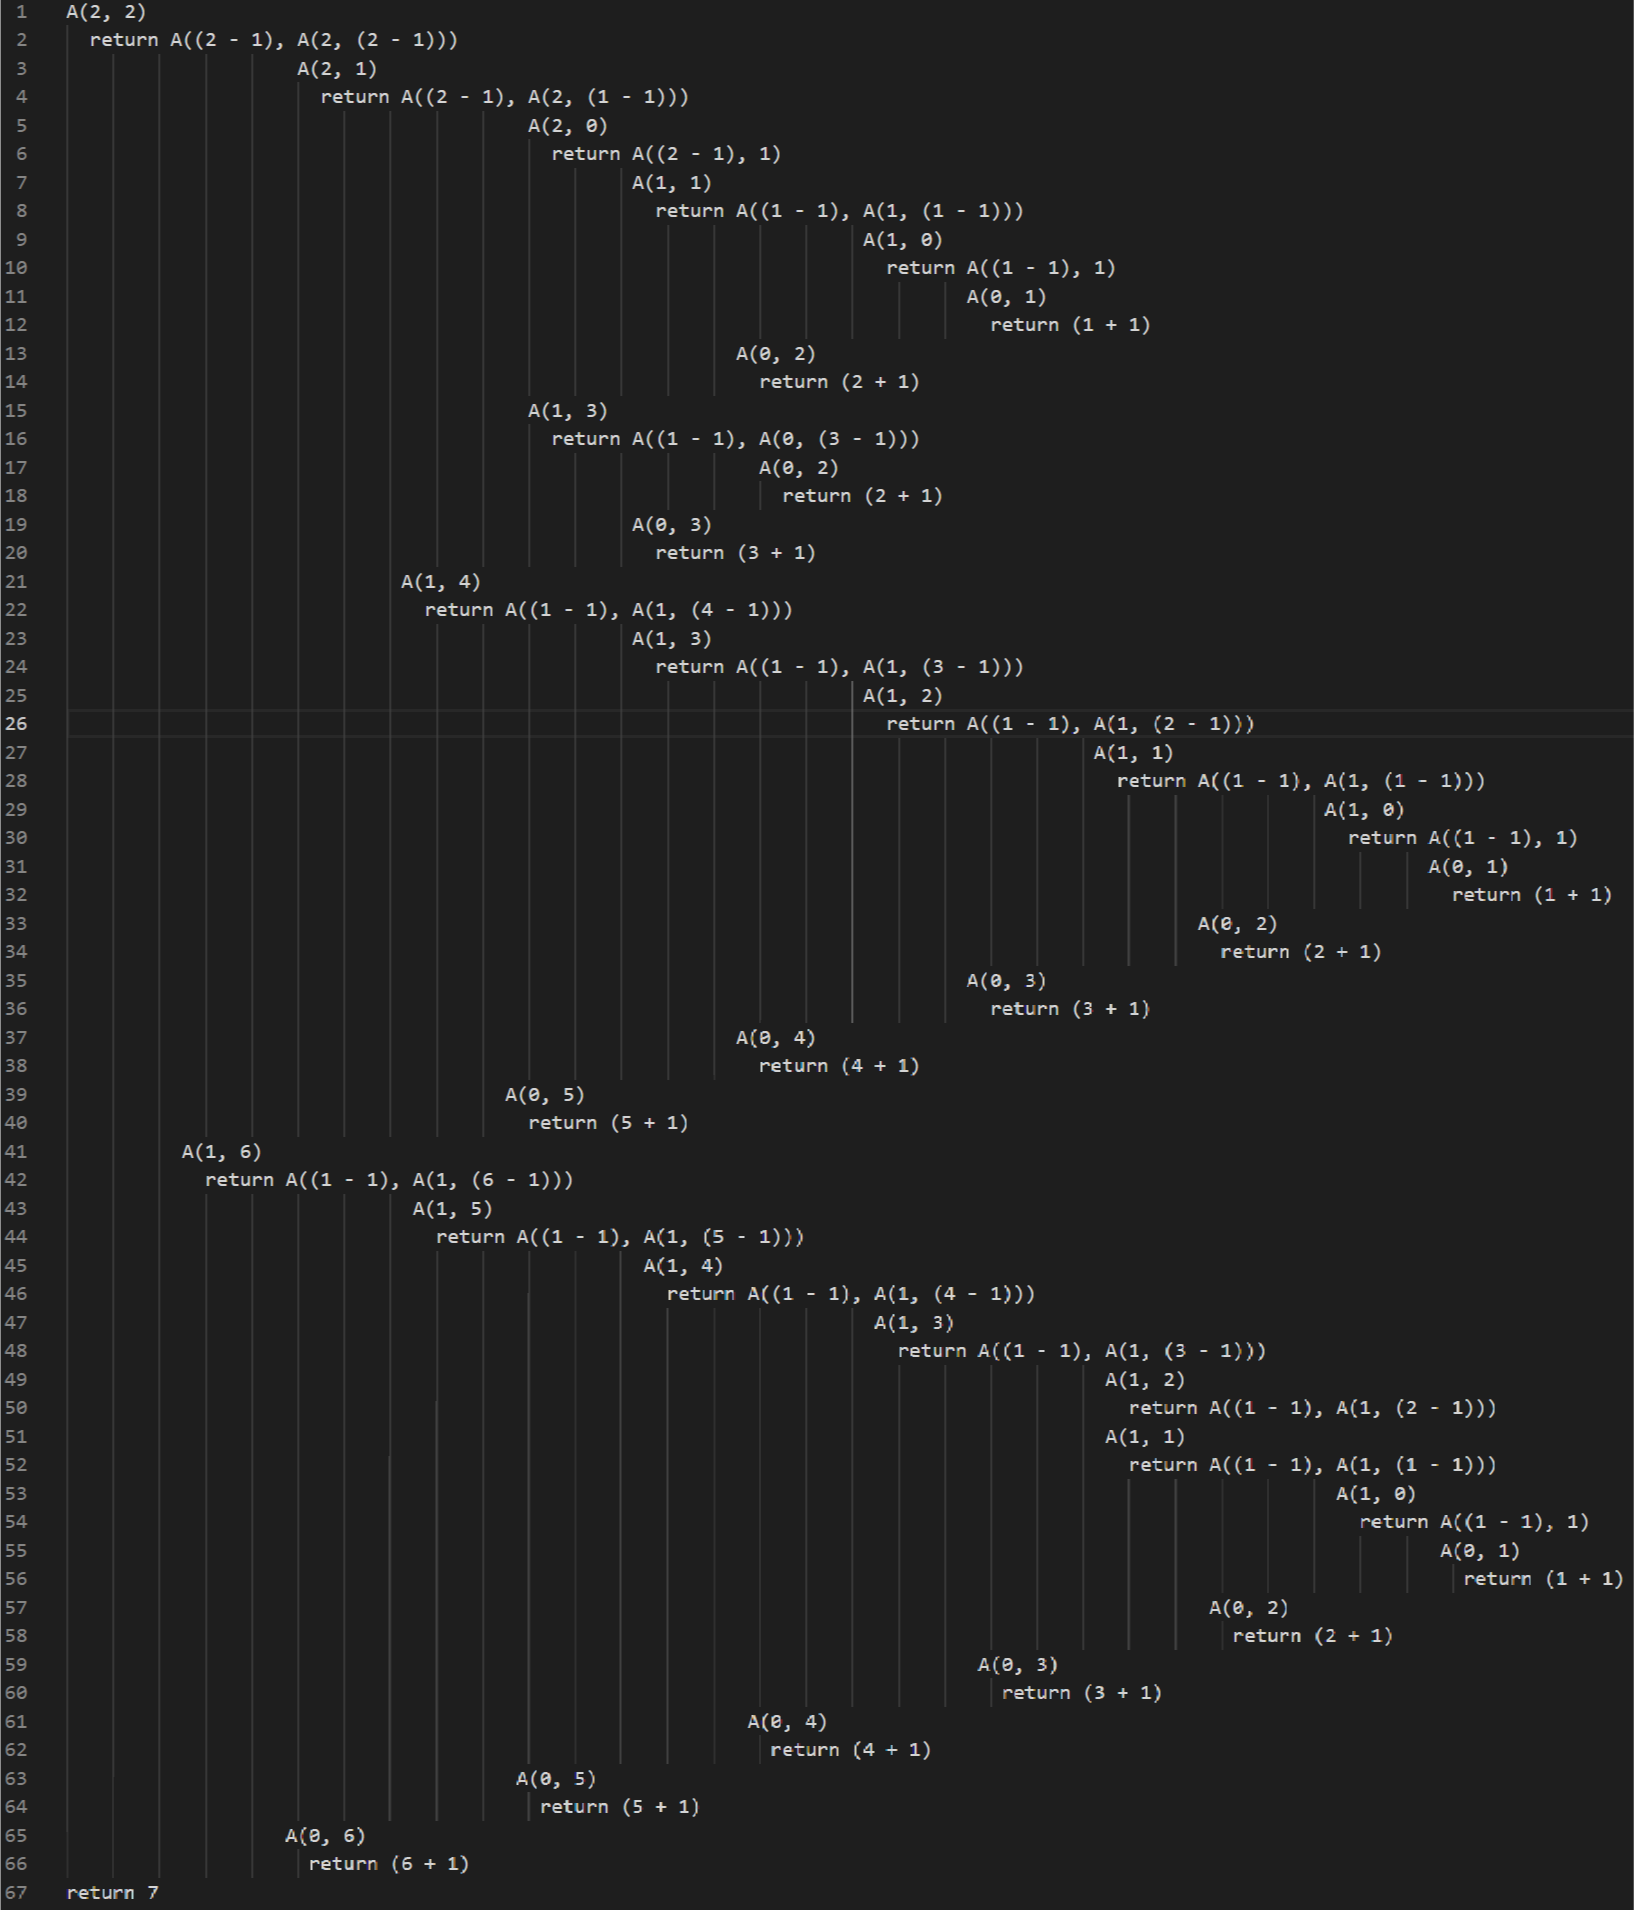
\includegraphics[width=\linewidth]{7.png}
    \linebreak
    Also it's correct that A(5, 5) gives a too many recusive calls error on my system however A(4, 4) works pretty fast.

    \item 
  \begin{lstlisting}
    # Problem 11
    def GCD(a, b):
        if 0 == a % b:
            return b
        return GCD(b, a % b)
    
    # Define GCD2    
    def GCD2(a, b, gcd = 0, s = 1, t = -1):
        if (a == b):
          return [a, 1, 0]            
        
        if (gcd == 0):
          gcd = GCD(a, b)
        
        d = (a * s) + (b * t)
        if (d == gcd):
            #print("Returning:", gcd, s, t)
            return [gcd, s, t]
        
        if (d > 0):
            t -= 1
        elif (d < 0):
            s += 1 
        
        #print("Returning GCD2(): ", a, b, gcd, s, t, "| d =", d)
        return GCD2(a, b, gcd, s, t)

    # Results
    print("Running GCD2 tests...\n")
    rand_a_range = [random.randint(1,2500) for i in range(10)]
    b = [random.randint(1,2500) for i in range(10)]
    results = []
    
    i = 0
    for a in rand_a_range:
        x = GCD2(a, b[i]) # Call GCD2(a, b).
        y = (x[1] * a) + (x[2] * b[i]) # Validate the results. 
        isValid = y == x[0]
        results.append([a, b[i], x, isValid, y])
        i += 1
        
    print(tabulate(results, headers=['a', 'b', 'GCD2() = [g, s, t]', 'Validated', 'GCD'], tablefmt='orgtbl'))    

    Running GCD2 tests...

    |    a |    b  | GCD2() = [g, s, t]   | Validated   |   GCD |
    |------+-------+----------------------+-------------+-------|
    | 1619 |  216  | [1, 107, -802]       | True        |     1 |
    |  360 |  240  | [120, 1, -1]         | True        |   120 |
    | 2233 |  377  | [29, 12, -71]        | True        |    29 |
    | 2315 |   16  | [1, 3, -434]         | True        |     1 |
    | 2442 | 1746  | [6, 143, -200]       | True        |     6 |
    |  788 | 1249  | [1, 233, -147]       | True        |     1 |
    | 2143 |  580  | [1, 367, -1356]      | True        |     1 |
    |  464 | 2280  | [8, 172, -35]        | True        |     8 |
    | 1166 | 1418  | [2, 377, -310]       | True        |     2 |
    |  286 | 1561  | [1, 846, -155]       | True        |     1 |
  \end{lstlisting}

  So essentailly my thought process is, first handle the stopping conditions one when a and b are equal in which case you know either one can be 1 and the other 0. Then the real stop condition we get the GCD if we don't have it yet then stop when the gcd equals our calcualtion of (a * s) + (b * t). Otherwise we check if we need to add to our negitive counter if essentailly if a - b is negitive or we add to our positive counter. Then we just keep recursivly calling till the calculation matches our gcd. Now it is pretty easy to high our recursion limit espically if the numbers have a small gcd and are large numbers.
  And to test I just generated some random numbers between 1 and 2500 for a and b and displayed the results.

  \item 
  \begin{lstlisting}
    # Problem 14
    def SuperReverse(l):
        if len(l) == 0:
            return
        elif len(l) == 1:
            if isinstance(l[0], list):
                return [SuperReverse(l[0])]
            return l
            
        return SuperReverse(l[1:]) + SuperReverse(l[:1])
        
    # Testing
    l = ['1', '2', '3', '4', '5']
    l2 = ['1', '2',['3.1', '3.2', ['3.3.1', '3.3.2'], '3.4'], '4', '5']
    print(SuperReverse(l))
    print(SuperReverse(l2))

    # Output    
    ['5', '4', '3', '2', '1']
    ['5', '4', ['3.4', ['3.3.2', '3.3.1'], '3.2', '3.1'], '2', '1']
  \end{lstlisting}

  \item 
  \begin{lstlisting}
    # Question 10
    def anagram2(st):
      if len(st) <= 1:
          return st

      lout = []
      
      for lout2 in anagram2(st[1:]):
          for i in range(len(st)):
              lout.append(lout2[:i] + st[0:1] + lout2[i:])
              
      return lout
  \end{lstlisting}
  \begin{lstlisting}
    # Testing
    lst = ['abcde', 'abcdef', 'abcdefg', 'abcdefgh', 'abcdefghi', 'abcdefghij', 'abcdefghijk']

    results = []
    for st in lst:
        t = time.time()
        ana = anagram(st)
        t = time.time() - t
    
        t2 = time.time()
        ana2 = anagram2(st)
        t2 = time.time() - t2
        
        diff = t2 - t
        
        results.append([t, t2, "{0:.6f}".format(diff), len(ana2)])
    
    headers = ['Runtime Anagram (sec)', 'Anagram2 (sec)', 'Time Difference', '# Anagrams']
    
    print(tabulate(results, headers, tablefmt='latex'))
  \end{lstlisting}
  \begin{tabular}{rrrr}
    \hline
       Runtime Anagram (sec) &   Anagram2 (sec) &   Time Diff &   \# Grams \\
    \hline
          0.099721   &       0.0937653  &   -0.005956 &       120 \\
          0.00196266 &       0          &   -0.001963 &       720 \\
          0.0139627  &       0.00199461 &   -0.011968 &      5040 \\
          0.108743   &       0.0179548  &   -0.090788 &     40320 \\
          1.00632    &       0.163535   &   -0.842788 &    362880 \\
         10.9808     &       1.6327     &   -9.34812  &   3628800 \\
        133.488      &      18.5607     & -114.927    &  39916800 \\
    \hline
    \end{tabular}
    
    So you can pretty easily tell from the table that the new "less" recursive Anagram2 algorithm is a good bit faster. Each algorithm roughly increases in line with the number of anagrams generated. If you look at the Aanagrams per milisecond on the base they stay faily consistantly around 330 for the origional and about 2,220 for the new one. So they both pretty much sacle to the number of anagrams generated. However due to how many more recursive calls the origional makes you'd expect it to reach it's recursion limit much sooner causes it to have a point where it'll never of almost all systems.

  \pagebreak
  \item Question 11
  \begin{enumerate}
    \item Australia.
    \item Facuality meeting.
    \item Phlisophy department at the university of Walamaloo.
    \item Five people, Michael and four Bruce's. 
    \item There is no rule \#6.
  \end{enumerate}

\end{enumerate}

\pagebreak
\begin{figure}
  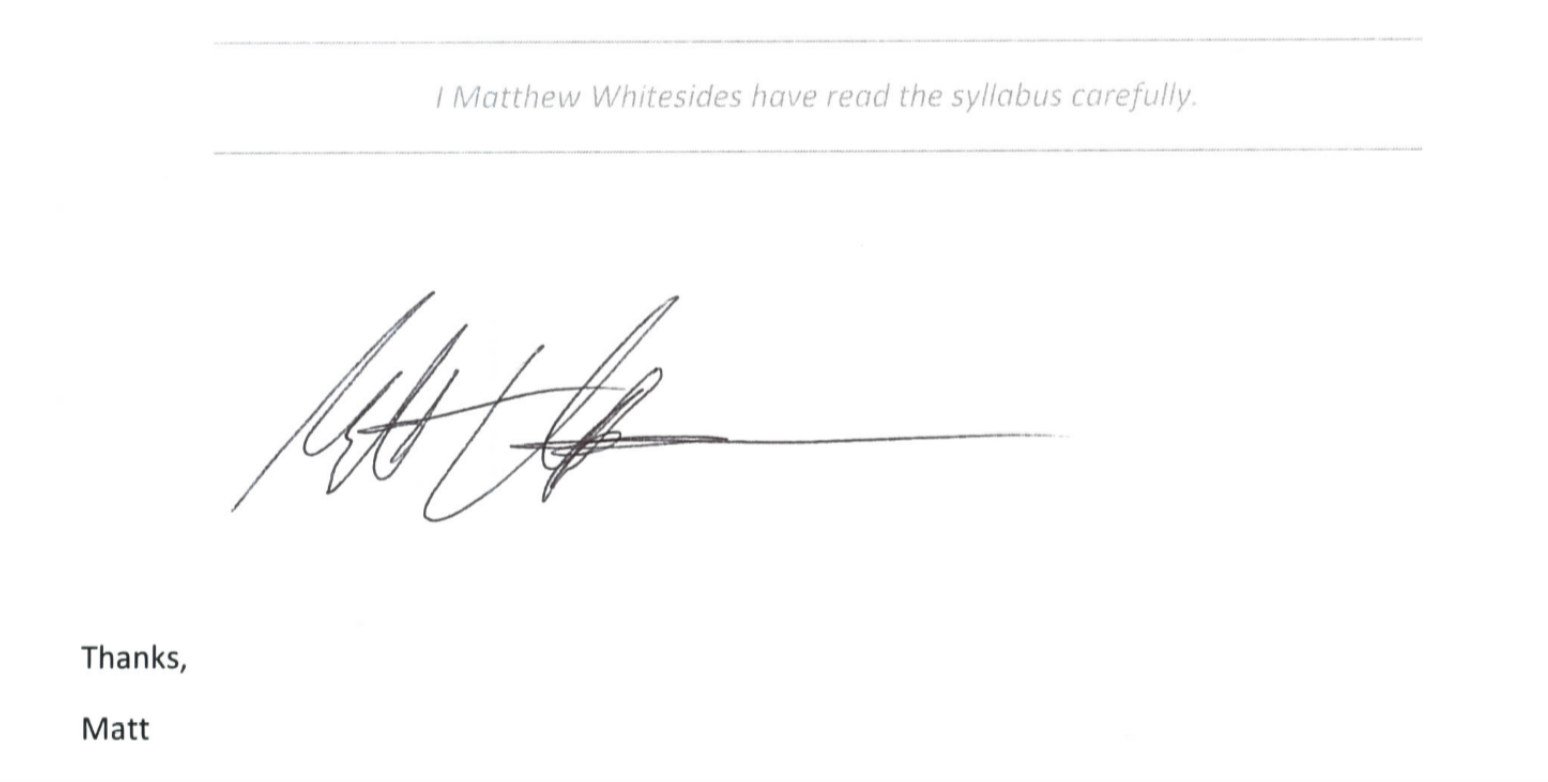
\includegraphics[width=\linewidth]{Statement.png}
  \label{fig:Statement}
\end{figure}

\end{document}
